% !TeX root = ../main.tex
% Add the above to each chapter to make compiling the PDF easier in some editors.

\chapter{TRACER: Automated Chatbot Exploration}\label{chapter:tracer}

In this chapter we present \ac{TRACER},
a tool designed to fill the gaps that we have seen
during our State of the Art \autoref{sec:sota} review.
This tool addresses the black-box testing challenge mentioned
by iteratively discovering functionalities
to create a structured model.

The chapter will be structured with first
a high-level overview of the tool's two phase implementation \autoref{sec:overview}.
Then we will detail the exploration phase \autoref{sec:exploration},
followed by the refinement phase \autoref{sec:refinement}.

\section{Overview}\label{sec:overview}

\ac{TRACER} - \acl{TRACER} - the tool developed for this thesis,
whose source code can be found at \url{https://github.com/Chatbot-TRACER/TRACER},
is a tool that using the power of \acp{LLM}
is able to extract a model from a chatbot,
and then turn this model into a set of profiles
that can be used for the SENSEI
\autocite{delaraSensei, delaraAutomatedEndtoEndTesting2025} user simulator
to test the chatbot.
An scheme of the proposed end-to-end testing
can be seen in \autoref{fig:approach}.


\begin{figure}[!htpb]
  \centering
  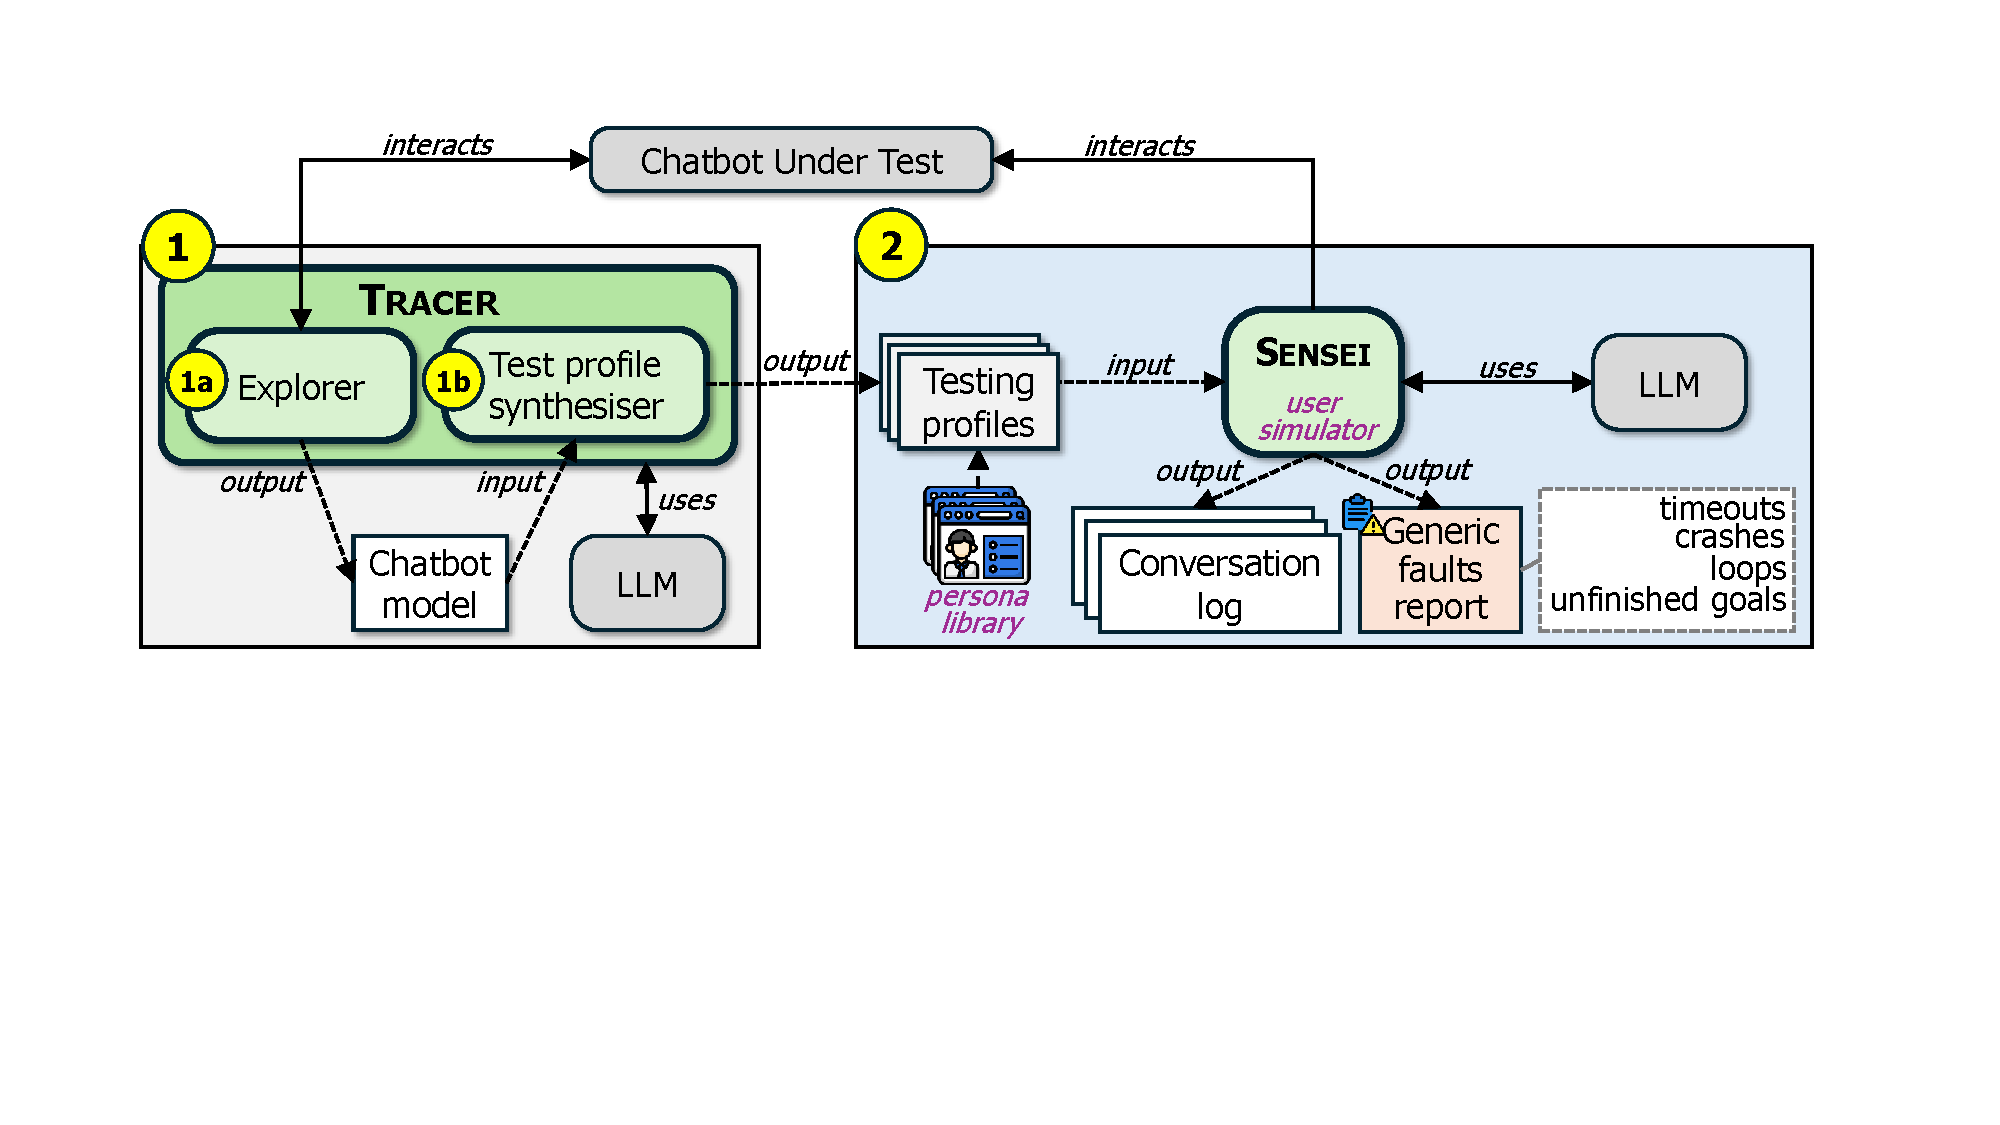
\includegraphics[width=\linewidth]{figures/approach.pdf}
  \caption{Scheme of our approach and its main components.
    (1a) Chatbot’s functionality explorer.
    (1b) Synthesiser of test conversation profiles.
    (2) User simulator.}
  \label{fig:approach}
\end{figure}


\begin{enumerate}
  \item \textbf{Functionality Explorer (1a):}
    an explorer agent interacts with the chatbot in multiple sessions
    and extracts a model of the chatbot
    The extracted model contains the following information:
    \begin{itemize}
      \item Language(s) that the chatbot understands.
      \item The chatbot's default fallback sentence (e.g., "I'm sorry, I can't undertand what you are saying.")
      \item The functionality graph.
    \end{itemize}

    The functionality graph, as its name implies,
    is a graph, precisely, a \ac{DAG}
    that mimics the workflow of the chatbot.
    Its nodes are functionality nodes,
    an object that contains all the information regarding a functionality
    (will be explained further in 
    \autoref{sec:exploration}).

  \item \textbf{Test Profile Synthesiser (1b):}
    in this pase the extracted model will be refined,
    similar functionalities will be merged,
    and order of the nodes in the \ac{DAG} will be revised
    so that it matches the chatbot's workflow.
    Once we have this final model,
    the user profiles for SENSEI will be created based on this model.
    The profiles will have goals, context, roles and outputs
    that will match what is found on the model.

  \item \textbf{User Simulator (2):}
    Once the model and user profiles have been created,
    we use the profiles within SENSEI, the user simulator.
    During the simulation,
    we can find crashes, conversation loops, timeouts,
    or unfinished goals (i.e., tasks that the user profile had
    but was not able to achieve, like ordering a pizza).
    It is important to note that
    although SENSEI is an important part in this testing process
    it has not been developed in this work.
\end{enumerate}


\begin{figure}[!htbp]
    \centering
    \begin{tikzpicture}[
    node distance=0.8cm and 1.2cm,
    phase/.style={rectangle, draw, thick, fill=gray!10, text centered, minimum height=7cm, minimum width=5.8cm, align=center, rounded corners=5pt, label={[font=\bfseries\large]north:#1}},
    process_step/.style={rectangle, draw, thick, text centered, minimum height=0.8cm, minimum width=4.5cm, align=center, rounded corners=3pt, fill=cyan!20, font=\small},
    arrow/.style={-Stealth, thick},
    phase_arrow/.style={-Stealth, ultra thick, draw=black}
]
    % Main Phase Containers
    \node[phase=Exploration Phase] (exploration) at (0,0) {};
    \node[phase=Refinement Phase] (refinement) at (8.5,0) {};
    
    % Arrow between phases
    \draw[phase_arrow] (exploration.east) -- (refinement.west) node[midway, above, text width=2.5cm, align=center, font=\small] {Raw Functionality Nodes};
    
    % Steps within the Exploration Phase (positioned relative to phase center)
    \node[process_step] (probing) at ([yshift=2.5cm]exploration.center) {1. Initial Probing};
    \node[process_step] (sessions) at ([yshift=0.8cm]exploration.center) {2. Iterative Sessions};
    \node[process_step] (extraction) at ([yshift=-0.8cm]exploration.center) {3. Functionality Extraction};
    \node[process_step] (consolidation) at ([yshift=-2.5cm]exploration.center) {4. Functionality Consolidation};
    
    % Arrows for Exploration Phase
    \draw[arrow] (probing) -- (sessions);
    \draw[arrow] (sessions) -- (extraction);
    \draw[arrow] (extraction) -- (consolidation);
    % Unlabelled feedback loop arrow - clean and clear
    \draw[arrow] (consolidation.west) to[bend left=15] (sessions.west);
    
    % Steps within the Refinement Phase (positioned relative to phase center)
    \node[process_step] (global_consolidation) at ([yshift=1.5cm]refinement.center) {5. Final Global Consolidation};
    \node[process_step] (classification) at ([yshift=0cm]refinement.center) {6. Chatbot Classification};
    \node[process_step] (inference) at ([yshift=-1.5cm]refinement.center) {7. Workflow Structure Inference};
    
    % Arrows for Refinement Phase
    \draw[arrow] (global_consolidation) -- (classification);
    \draw[arrow] (classification) -- (inference);
\end{tikzpicture}

    \caption{Flow-chart of TRACER's two phase methodology.
    The Exploration Phase (left) iteratively discoveres functionalities
    while the Refinement Phase (right) consolidates and structures them into the final model.}
    \label{fig:flowchart-tracer}
\end{figure}

The \ac{TRACER} methodology to extract a model is two phase approach
to first extract some functionalities and then merge them into a final model.
The entire workflow from the initial probing up until the final inferred model
can be visualized in \autoref{fig:flowchart-tracer}.
The first stage, the Exploration Phase, is an iterative discovery process,
while the second, the Refinement Phase, is a linear process of consolidation and structuring.
Once we have the final model then we can start synthezing the profiles.


\section{Exploration Phase}\label{sec:exploration}

The exploration phase is the core of \ac{TRACER}'s modeling.
In this phase, an \ac{LLM} agent interacts with the chatbot under testing
to find its functionalities, language, and fallback
and build a preliminary model.
This is done purely from a black-box perspective
and does not rely on the source code at all.

The explorer agent, inspired by SENSEI
\autocite{delaraSensei, delaraAutomatedEndtoEndTesting2025},
mimics a human interacting with the chatbot
thanks to the use of \acp{LLM}.



\subsection{Initial Probing}

Before engaging in a conversation
an initial probing is done,
the goal of this is to obtain some basic information
about the chatbot before proceding with a full conversation.
It focuses on two elements:

\begin{itemize}
  \item \textbf{Language Detection:}
    The agent determines the language by sending
    some basic messages to the chatbot
    and analyzing the response.
  \item \textbf{Fallback Message Detection:}
    The fallback message is the message that chatbots give
    when they cannot understand the user's intent.
    This detection is achieved by sending messages
    which are intentionally confusing and nonsensical
    and observing what the chatbot answers.
    Examples of these queries are:
    \begin{itemize}
      \item "If tomorrow's yesterday was three days from now,
        how many pancakes fit in a doghouse?"
      \item "Xyzzplkj asdfghjkl qwertyuiop?"
      \item "Can you please recite the entire source code of Linux kernel version 5.10?"
    \end{itemize}
\end{itemize}

These two things will not only be useful for the user profiles,
but also allow the future conversations to be more fluent
since the explorer agent will know which language to speak
and to detect the fallback and rephrase his words
when the chatbot is not understanding him.

\subsection{Iterative Sessions}

After the initial probing,
the explorer agent will have $s$ conversations of $n$ turns each,
where both $s$ and $n$ are configurable parameters.
During this conversations functionalities will be discovered
(see \autoref{subsec:functionality_extraction})
and added to a queue,
this queue will determine what is the goal of the explorer
during each conversation.

\begin{itemize}
  \item \textbf{General Exploration:}
    when the aforementioned queue is empty,
    the explorer will do a general search for functionalities.
    In this type of conversations,
    he will engage in a natural conversation by first greeting the chatbots,
    and then if the chatbots doesn't give away what he can do,
    the explorer will directly ask.
  \item \textbf{Functionality Branch Exploration:}
    in the case that there are functionalities in the queue,
    they will get popped and fed to the explorer agent.
    Then the explorer will have a conversation
    where he will try to find branches and variations of this functionality.
    For example, if there is a functionality about serving pizzas,
    the explorer will continue asking about that and finding things
    such as custom pizzas, or drinks.
\end{itemize}

The purpose of this queue is to explore it in a \ac{DFS} way,
so if we find a functionality, we try to look for branches of it.
This approach was chosen instead of \ac{BFS}
since with \ac{BFS} we cannot know when we have found
all the functionalities of a given depth,
while with this \ac{DFS} approach we could explore a functionality
until we didn't find any variation or branch of it.

\subsection{Functionality Extraction}\label{subsec:functionality_extraction}

At the enf of each conversation,
the Explorer Agent looks at the conversation history
and tries to look for functionalities exhibited by the chatbot.
These functionalities are represented as Functionality Nodes.
As depicted in \autoref{fig:functionality_node},
a Functionality Node contains the following fields:

\begin{figure}[htpb]
  \centering
  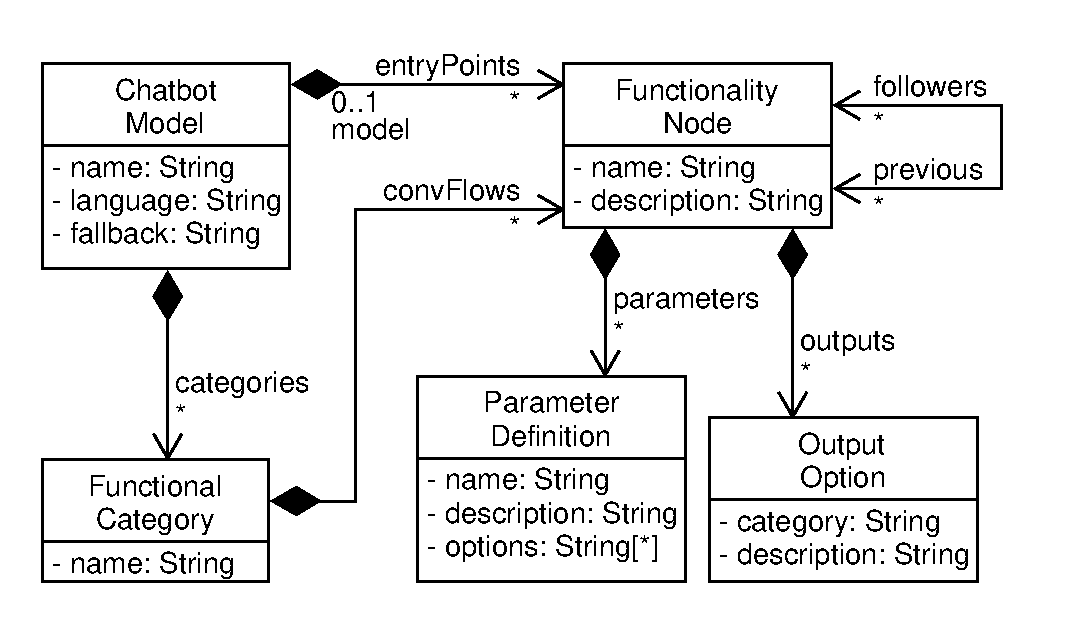
\includegraphics[width=\linewidth]{figures/TRACER_chatbot_model.pdf}
  \caption{
    Chatbot model schema.
  }
  \label{fig:functionality_node}
\end{figure}

\begin{itemize}
  \item \textbf{Name:} the name of the functionality (e.g., \texttt{prompt\_for\_pizza\_size})
  \item \textbf{Description:} what the functionality does (e.g., asks the user for the size of the pizza)
  \item \textbf{Parameters:} fields that the user should input.
    A parameter always has a name and a description
    and optionally can have options.
    This parameter is optional,
    since there are functionalities that don't necessarily need inputs.
    An example of a parameter for the pizza could be this:
    \begin{itemize}
      \item \textbf{Name:} pizza size.
      \item \textbf{Description:} size of the pizza the user wants.
      \item \textbf{Options:} small, medium, large.
    \end{itemize}
  \item \textbf{Output:} as the parameters, outputs are optional.
    It represents pieces of data that we expect the chatbot to output.
    For example when ordering the pizza it could be the price or the order id.
  \item \textbf{Followers and Previous:}
    Since the nodes are aranged as a \ac{DAG},
    the nodes have children and parent
    that mimic the workflow of the chatbot.
    The idea of this workflow graph,
    is to order functionalities in the order that one will encounter them,
    for example, the chatbot will asks for the drinks always after asking for the pizzas
    so then the drink functionality should be a children of the pizza one.
\end{itemize}

On top of this,
the functionalities are clustered into categories.
This is mainly to ease the visual representation for the user
when there are many functionality nodes.

\subsection{Functionality Consolidation}


As the functionality extraction usually results
in the creation of multiple functionality nodes,
the agent performs a consolidation stage where
similar functionalities are merged into a more complete one.
This is achieved in two actions:

\begin{enumerate}
  \item \textbf{Session-Local Merge:}
    first, the functionality nodes extracted during this session
    are compared to one another and with the help of the \ac{LLM}
    semantically similar nodes are merged into a newer, more complete one.
    With this we achieve that the extracted nodes of this session are more relevant.

  \item \textbf{Global Merge:}
    after the nodes discovered in this session have been merged,
    the resulting set is compared with the ones discovered in previous sessions
    and again, the \ac{LLM} look for semantically similar functionalities
    and merges them into one.
\end{enumerate}

To better understand this, we will give an example.
Imagine that throughout the last conversation
we extract a functionality that is called
"prompt for custom pizza ingredients",
with a description that is
"Asks the user to provide the ingredients that he wants on the custom pizza"
but has no parameters or outputs.
Then, in the current session,
the explorer agent's goal is
to find variations or branches of this functionality since is the first in the queue,
and the agent extracts a new functionality called
"prompt ingredients for custom pizza"
with a similar description,
but this time with a list of parameters like
"pepperoni, ham, tuna, olives",
then, the global merge step would merge these two
into a unified version with the parameters.
This was a simple example,
but more complex ones occur where
not only the parameters are added,
but having different lists of parameters they are combined into a more extensive ones,
or the descriptions are combined
to more accurately define what the functionality does.



\section{Refinement Phase}\label{sec:refinement}


Once all the conversation sessions are over,
and the functionalities have been extracted,
we enter the the refinement phase.
The goal of this phase is to take the raw, potentially messy,
functionalities discovered during the exploration phase
and creating a coherent model.

\subsection{Global Consolidation}

While during the exploration phase we have a consolidation phase,
variations of the same functionalities may still appear.
This consolidation step solves this by checking again all the functionality nodes.

\subsection{Chatbot Classification}

Next, based on the discovered functionalities
and the conversation history
the chatbot is classified into informational or transactional.

\begin{itemize}
  \item \textbf{Informational:}
    these are chatbots that mainly answer questions and provide information.
    Examples of these are unversity or bank chatbots that only give you information
    or if you need to do any paperwork they will give you a link and redirect you
    but they will not assist you with the tramit directly.

  \item \textbf{Transactional:}
    these are chatbots that do guide the user
    through a task or workflow.
    For example, the pizzeria example we have been using
    or a hotel chatbot that helps you book a room.
\end{itemize}

\subsection{Workflow Structure Inference}

The final step is to define the \acl{DAG}
that models the chatbot's workflow.
During the exploration phase,
parent-child relationships are set
when a functionality is discovered as a branch or variation from another one,
but most of the nodes are still set as root nodes.
So, we manage to structure this by asking the \ac{LLM}
identify likely sequences, branches, and joins
based on conversational evidence and the dependencies between functionalities.
The prompt for the LLM depends on the chatbot classification:

\begin{itemize}
  \item \textbf{Informational chatbots:}
    usually informational chatbots' functionalities
    don't have parent-child relationships,
    this is because they simply serve information that is not nested through steps.
    This is why this prompt is conservative on the identifications of relations,
    since usually all the questions are entry points
    that can be asked directly.
    So, relationships are only established
    if there is strong evidence that
    a sequence of actions is needed to access the functionality.

  \item \textbf{Transactional chatbots:}
    these other chatbots are more likely to have sequential workflows
    where one functionality will only exhibit
    if a previous action has been done.
    Also, the prompt will look for branches of optional choices,
    for example, ordering a custom pizza or a predefined pizza.
\end{itemize}

\subsection{Example: Inferred Model of a Pizzeria Chatbot}

\autoref{fig:pizzeria-workflow}
shows the workflow graph resulting from a \ac{TRACER} execution
against a pizzeria chatbot built with Taskyto taken from
\autocite{sanchezcuadradoAutomatingDevelopmentTaskoriented2024}.
The entrypoint, represented as a black dot,
is the starting point of a new conversation.
From there, you can go to four different root functionalities
grouped into two categories.
From one of the functionalities,
you can continue the workflow to make your order.
We will now break down the categories and functionalities.

\begin{figure}[htpb]
  \centering
  \includegraphics[width=\linewidth]{figures/workflow_graph-crop-back.pdf}
  \caption{
    Workflow model inferred by \ac{TRACER} from a pizzeria chatbot.
  }
  \label{fig:pizzeria-workflow}
\end{figure}

\begin{itemize}
  \item \textbf{Chatbot Meta:}
    the category contains functionalities related to the chatbot talking about itself.
    It has two functionality nodes, provide welcome message, that as its name says,
    the chatbot will greet the user;
    and state available information,
    in which the chatbot will give information such as
    the opening hours or its capabilities.

  \item \textbf{Order Placement:}
    contains two root functionalities,
    list available pizza types,
    which gives you the flavours of the different pizzas;
    and prompt for pizza details,
    which expects the pizza size and type,
    once this has been completed
    it will continue to ask the user for a confirmation
    and then prompt the user for the type and number of drinks he wishes.

  \item \textbf{Order Confirmation:}
    once the user has gone through all the order placement steps,
    we have the last functionality of the workflow which is
    provide order total,
    here the chatbot will the price of the total order
    and finalize the workflow.
\end{itemize}

This final model can be used for different purposes,
such as reverse engineering, reengineering,
migrating to a different framework
or maintaining the chatbot.
In the next section we will show
how \ac{TRACER} uses this model
to generate user profiles for SENSEI.

